\newpage
\section{THEORETICAL BACKGROUND}
\subsection{General}
The project tries to study the impact of the personality on the collaborative recommendation engine. Thus, initially personality of the user has to be predicted which can be done via the user's study on social media i.e Facebook where a status update might be one of the good metric to predict the personality using \textbf{"document classification"} technique and the traits of the person are used as the similarity metric for similar user computation on \textbf{"collaborative filtering"}.

\subsection{Document Classification}
Document Classification is an example of Machine Learning(ML) in the form ofNatural Language Processing(NLP). By classifying text, we are aiming to assign one or more classes or categories to a document, making it easier to manage or sort.
Broadly speaking, there are two classes of ML techniques:
\begin{enumerate}
\item Unsupervised: In unsupervised method, model is responsible for clustering of a similar document.
\item Supervised: In supervised methods, a model is created based on training set. Categories are predefined and documents within the training dataset are manually tagged with one or more category labels. A classifier is then trained on the dataset which means it can predict a new document's category from then on. "This is the technique that has been used in the project."
\end{enumerate}

Supervised Document Classification comprises of series of steps which are briefly described below:
\subsubsection{Obtaining a dataset}
The quality of the tagged dataset is by far the most important component of a statistical NLP classifier. The dataset needs to be large enough to have an adequate number of document in each class. The datasets also needs to be of a high enough quality in terms of how distinct the documents in the different categories are from each other to allow a clear delineation between categories \cite{kd}.

\subsubsection{Preprocessing}
Preprocessing or Data preprocessing is a data mining technique that involves transforming raw data into an understandable format(as per requirement of the project may differ from the need of the project).
It comprises of various steps:
\begin{itemize}
\item Data Cleaning: Data is cleansed through processes such as filling in missing values, smoothing the noisy data or resolving the inconsistencies in the data.
\item Data Integration: Data with different representation are put together and conflicts within the data are resolved.
\item Data Transformation: Data is normalized, aggregated and generalized.
\item Data Reduction: This step aims to present a reduced representation of the data in a data warehouse.
\item Data Discretization: This involves the reduction of a number of values of a continuous attribute by dividing the range of attribute intervals. \\
\end{itemize}
The preprocessing carried out in the project are:
\begin{enumerate}
\item Removal of StopWords:
In computing, stop words are words which are filtered out prior to, or after processing of natural language data(text). There is not one definite list of stop words which all tools use and such a filter is not always used. Any group of words cab be chosen as the stop words for a given purpose. By removing the stop words during data preprocessing we reduce the computational complexity of the program and hence the project can run in an effective way \cite{stopwords}.
\item Convert every characters to lowercase:
This step is carried out in order to remove the distinction between the same words written in upper and lower case, so that model doesn't treat them differently.
\item Sentence level processing/tokenization:
In lexical analysis, tokenization is the process of breaking a stream of text up into words, phrases, symbols or other meaningful elements called tokens. Here in the project sentences are tokenized into the words and some more preprocessing are applied after that.
\item Stemming:
In linguistic morphology and information retrieval, stemming is the process for reducing inflected(or sometimes derived) words to their stem, base or root form generally a written word form. The stem need not be identical to the morphological root of the word. It is usually sufficient that related words map to the same stem, even if this stem is not itself a valid root. It is generally a implemented as the rule based system for stemming for words \cite{porter}.
\item PoS tagging:
In corpus linguistics, a part of speech tagging, also called grammatical tagging or word-category disambiguation, is the process of marking up a word in a text(corpus) as corresponding to a particular part of speech, based on it's definition as well as context i.e relationship with adjacent and related words in a phrase, sentence, or paragraph \cite{pos}. This aids in removal of unwanted part of speech in the sentences and helps to build the better model. The parts of speech used in our model are verb, adverb and adjective.
\end{enumerate}

\subsubsection{Feature Extraction}
\begin{enumerate}
\item Bag of Words:
 The bag of words model is a simplifying representation used in natural language processing and information retrieval(IR). In this model, a text (such as sentence or a document) is represented as the bag disregarding grammar and even word order but keeping multiplicity. The bag of words model is commonly used in methods of document classification where the frequency or occurrence of each word is used as a feature for training a classifier. It is comparable to the skip gram model of the unigram in the language model \cite{vector}

% \item Term Frquency - Inverse Document Frequency(TF-IDF):
% TF-IDF \cite{tfidf} is a common term weighting scheme. It is a statistical approach to evaluating the importance of term in a corpus. Typically tf-idf weight is composed by two terms: the first computes the normalized Term Frequency(TF) i.e the number of times a word appears in a document, divided by the total number of words in that document, the second term is the inverse doucment frequency(IDF) computed as the logarithm of the number of documents in the corpus divided by the document length i.e total number of terms in the document as a way of normalization.

% i.e
% \begin{equation}
% \begin{split}
% 	TF = \frac{Number of times term t appears in a document}{Total number of terms in the document} \\
% 	IDF = \log_e\frac{Total number of documents}{1+Number of documents with term t in it} \\
% \end{split}
% \end{equation}
% Now tf-idf can be obtained as:
% \begin{equation}
% 	TF-IDF = tf * idf
% \end{equation}
\item Feature Vector Creation:
 Feature Vector Creation is the process of conversion of bag of words model of into the vector form where by each words are represented with their frequencies. For feature vector creation initially a vocabulary is built using all of the corpus available in dataset which helps to create a vector space model for words and feature vector are derived from the each corpus accordingly \cite{vector}.
\end{enumerate}

\subsubsection{Model Creation}
It is a classification algorithm used for the classification of personality in the project. Here we have implemented Naive Bayes, Logistic Regression as the classification algorithm.
%\begin{itemize}
% \subsubsection{ kNN(k-Nearest Neighbors)}
% It is a one of the simplest non-linear classification alogrithm with no model and is also known as lazy classifier. By lazy classifier, it means that while training, it does not dow much expect for storing the data points. kNN looks to classify data only when the new data is given as input for the prediction. It takes k nearest neighbors, to the given input data and then decides which class it belongs to via majority voting. Nearest neighbors are found out through a predefined distance function.In the project consine similarity is used as the metric to compute how similar is input feature vector to the existing one in the database.\\

% The brief outline of the algorithm is given below:
% \begin{enumerate}
% 	\item Calculate the distance or dissimilarity or similarity of the given input point with all other points.
% 	\item Select k-nearest points from the given data point.
% 	\item Count the distinct classes of the k-nearest point and assign the class with the maximum count to the given data point.

% 	The algorithm uses different dissimilarity or similarity measures for different kinds of attributes of data. In the project, cosine similarity metric has been used in order to find out similar k-neighbors.

% Suppose $r_a = [r_a1,r_a2,\cdots,r_an]$ be the feature vector of the document a and  $r_b = [r_b1,r_b2,\cdots,r_bn]$ be the feature vector of the document b, then cosine similarity between document a and b can be obtained as:
% \begin{equation}
% 	similarity_{a,b} = \frac{r_a1*r_b1 + r_a2*r_b2 +\cdots+ r_an*r_bn}{\sqrt{{r_a1}^2+{r_a2}^2+\cdots+{r_an}^2} * \sqrt{{r_b1}^2+{r_b2}^2+\cdots+{r_bn}^2} }
% \end{equation}
% which is used as the metric to compute the $k$ similar document.
% \end{enumerate}
\subsubsection{ Logistic Regression}
In general, when we make a machine learning based software, we are basically
trying to come up with a function to predict the output for future inputs based
on the experience it has gained through the past inputs and their outputs.
The past data is referred to as the {\em training set}.

{\bf Logistic regression}\cite{ng} (also known as {\em logit regression} or {\em logit model}) is one of
the most popular machine learning algorithms used for classification problem.
Given a training set having one or more independent (input) variables where
each input set belongs to one of predefined classes (categories), what
logistic regression model tries to do is come up with a probability function
that gives the probability for the given input set to belong to one of those
classes. The basic logistic regression model is a binary classifier (having
only 2 classes), i.e., it gives the probability of an input set to belong to
one class instead of the other. If the probability is less than 0.5, we can
predict the inputs set to belong to the latter class. But logistic regression
can be hacked to work for multi-class classification problem as well by using
concepts like ``{\em one vs. rest}''. What we basically do is create a classifier for
each class that predicts the probability of an input set to belong to that
particular class instead of all other classes. It is popular because it is a
relatively simple algorithm that performs very well on wide range of problem
domains.

Actually, logistic regression is one of the techniques borrowed by machine
learning from the field of statistics. Logistic regression was developed by
statistician David Cox in 1958. The binary logistic model is used to estimate
the probability of a binary response based on one or more predictor
(or independent) variables (called {\em features}).

The name ``{\em logistic}'' comes from the probability function used by this algorithm.
The logistic function (also known as {\em sigmoid} function) is defined as:
\begin{align}
  \text{logistic}(x) = \text{sigmoid}(x)
  = \frac{e^x}{1 + e^x}
  = \frac{1}{1 + e^{-x}} \label{eqn:logit}
\end{align}

The graph of this function is given in Figure \ref{fig:sigmoid}.
\begin{figure}[h!]\centering
  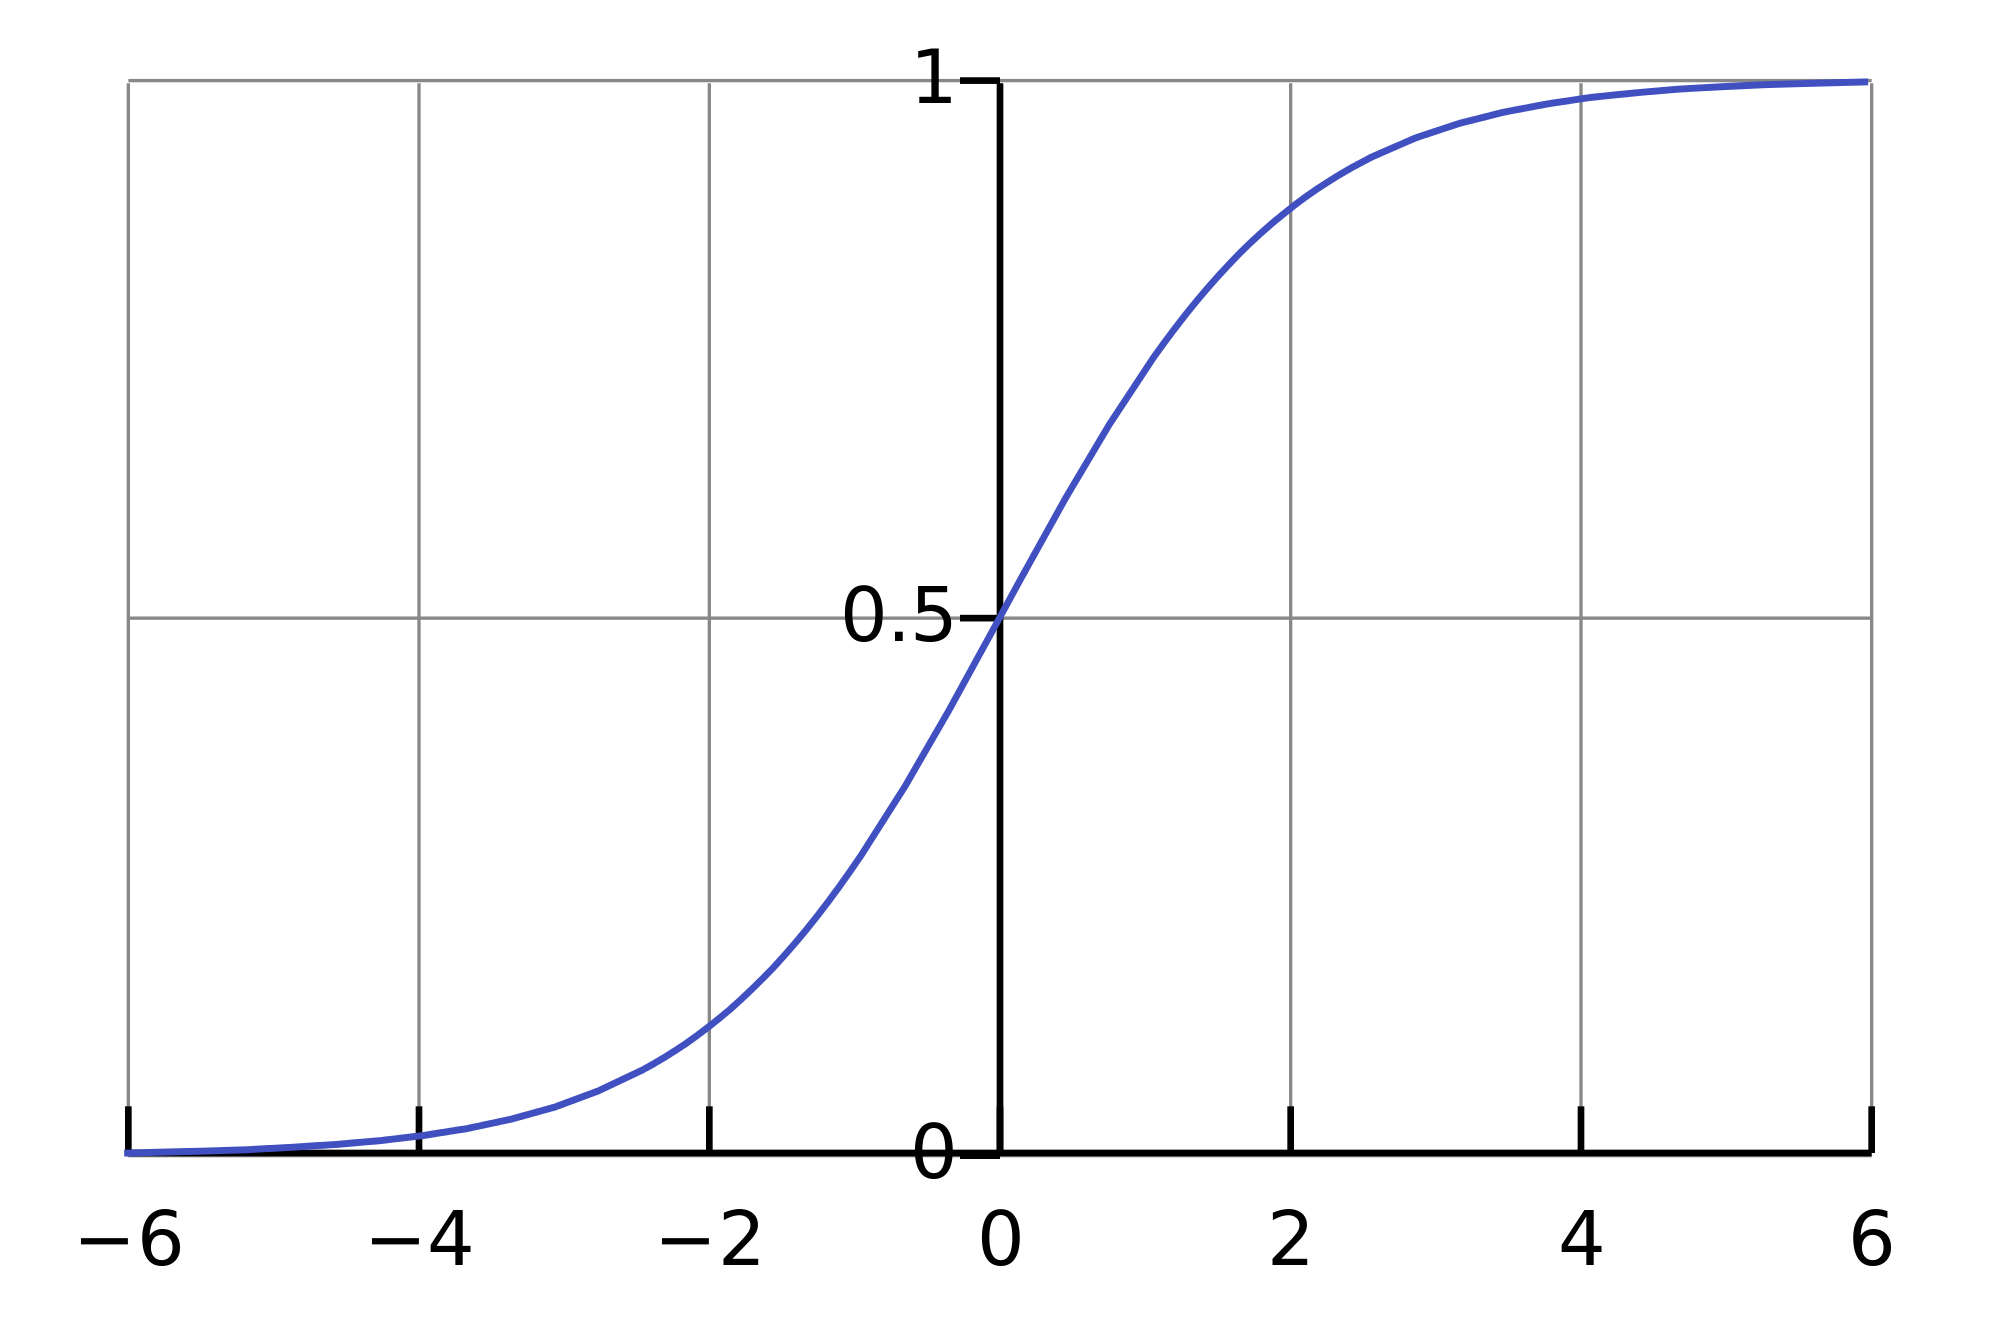
\includegraphics[width=3in]{fig/sigmoid}
  \caption{Graph of logistic (sigmoid) function}\label{fig:sigmoid}
\end{figure}

The logistic regression classifier uses the logistic function of the {\em weighed}
(as well as biased) sum of the input variables to predict the probability of
the input set belonging to a class (or category). The probability function is
already fixed. The only thing that we can change while learning from different
training set is the set of weight parameters ($\theta$) assigned to each feature.

\paragraph{The Algorithm}\hfill

Let,
\begin{align}
  m &= \text{number of samples in training set}
  \nonumber\\
  n &= \text{number of features} \ge 1
  \nonumber\\
  x &= \text{input feature vector} =
  \begin{bmatrix}
  x_0 \\ x_1 \\ x_2 \\ \vdots \\ x_n
  \end{bmatrix}, x_0 = 1 \text{(always)}
  \nonumber\\
  y &= \text{class} \in \{ 1, 0 \} \text{ with 1 as primary class}
  \nonumber
\end{align}

The training set for this machine learning algorithm is the set of $m$ training
samples (examples).
\begin{align}
  \text{training set} =
  \left\{ (x^{(1)}, y^{(1)}), (x^{(2)}, y^{(2)}), \cdots , (x^{(m)}, y^{(m)}) \right\}
  \label{eqn:training-set}
\end{align}

The weight parameters for the $(n+1)$ features are given by:
\begin{align}
  \theta =
  \begin{bmatrix}
    \theta_0 \\ \theta_1 \\ \theta_2 \\ \vdots \\ \theta_n
  \end{bmatrix}
  \nonumber
\end{align}

Then the hypothesis function used to predict the output $y$ for
input feature set $x$ with parameter $\theta$ is given by:
\begin{align}
  \text{h}_{\theta}(x) =
  \text{sigmoid}\left( \sum_{i = 0}^{n} \theta_{i} x_{i}\right) =
  \text{sigmoid}\left( \theta^{T}x \right) =
  \frac{1}{1 + e^{-\theta^{T}x}}
  \label{eqn:hypothesis}
\end{align}

Now the aim of this machine learning algorithms is to adjust the parameters
$\theta$ to fit the hypothesis $h_{\theta}(x)$ with the real output $y$ of
training set with minimum cost (error). For that, we need to define the cost
function, preferably, a {\em convex} cost function. There are different types
of cost functions. Linear regression, for instance, uses the sum of the squares
of the errors as the cost function. But in logistic regression, since the output
is not linear (even though the input is), this cost function turns out to be
non-convex and there are not efficient algorithms that can minimize a non-convex
function. Therefore, we define a logarithmic cost function $J(\theta)$ for logistic regression
as follows:
\begin{align}
  \text{J}(\theta) = \frac{1}{m} \sum_{i=1}^{m}
  \text{Cost} \left( \text{h}_\theta \left(x^{(i)} \right), y^{(i)} \right)
  \label{eqn:j}
\end{align}
where,
\begin{align}
  \text{Cost} (h, y) &=
  \begin{cases}
    -\log (h) &\text{ for } y = 1 \\
    -\log (1-h) &\text{ for } y = 0
  \end{cases}
  \nonumber\\
  &= -y\log(h) - (1-y)\log(1-h)
  \label{eqn:cost}
\end{align}

After we define an appropriate convex cost function J($\theta$), the machine
learning algorithm basically boils down to finding parameter $\theta$
that minimizes J($\theta$).
\begin{align}
  \min_{\theta} \quad \text{J}(\theta)
\end{align}

This can be achieved using various optimization algorithms. Some notable
ones are Gradient descent, BFGS, Quasi-Newton, L-BFGS, etc. The gradient
descent is the simplest one. It is a hill-climbing optimization algorithm
that tries finds the local optima from the start point. But since our
cost function J($\theta$) is convex, there is only one minima and that is the
global minima.

To find parameter $\theta$ that minimizes the cost function J($\theta$),
we initial $\theta$ with small random values and then
iterate the following until convergence:
\begin{align}
  \theta_j = \theta_j - \alpha \frac{\partial \text{J}(\theta)}{\partial \theta_j};
  \quad j \in {0,1,2,\ldots,n}; \quad \alpha = \text{learning rate}
  \nonumber
\end{align}
where,
\begin{align}
  \frac{\partial \text{J}(\theta)}{\partial \theta_j} =
  \sum_{i=1}^{m} \left( \text{h}_\theta \left(x^{(i)}\right) - y^{(i)} \right) x^{(i)}_j
\end{align}
Note that all $\theta_j$'s must be updated simultaneously. This concept is called
{\em batch learning}, contrary to {\em online learning} where the parameter is updated
separately for every training example.

The resulting parameter $\theta$ that minimizes the cost function J($\theta$) is
the parameter of the learning model. Then we can use the hypothesis $h_\theta(x)$
to predict the output $y$ for any input feature set $x$. The output $y$ will be
a value in the range $(0,1)$. The output can be interpreted as the probability
of the given input set belonging to the class 1 (primary class).

Other advanced optimization algorithms such as BFGS, L-BFGS, Quasi-Newton, etc.
are more efficient that the basic gradient descent and also has the advantage that
we don't have to manually select the learning rate ($\alpha$). These advanced
optimization algorithms will automatically select the appropriate value of $\alpha$
to maximize efficiency.

\paragraph{Other Considerations}\hfill


\subparagraph{Feature Scaling}\hfill

Feature scaling is the process of scaling (or normalizing) all the features
to a limit of $[-1,1]$ or $[0,1]$. This is required because unscaled features
causes some features to get higher priority implicitly and it reduces
the accuracy of the learning algorithm. Feature scaling can be done in following
ways:
\begin{align}
  x_j^{(i)} &= \frac{x_j^{(i)} - \min (x_j)}{ \max (x_j) - \min (x_j)}
  \in [0, 1]
  \nonumber
\end{align}
or
\begin{align}
  x_j^{(i)} &= \frac{x_j^{(i)} - \overline{x_j}}{ \max (x_j) - \min (x_j)}
  \in [-1, 1]
  \nonumber
\end{align}
or
\begin{align}
  x_j^{(i)} &= \frac{x_j^{(i)} - \overline{x_j}}{\sigma_{x_j}}
  \quad (\text{for normal distribution})
  \nonumber
\end{align}


\subparagraph{Regularization}\hfill


Regularization \cite{jason} is the process of scaling down the values of parameter $\theta$
to reduce the problem of over-fitting. Over-fitting is the condition when
the learning algorithm satisfies the training set very precisely but doesn't
satisfy test data (not included in training set). Regularization is done
by introducing a regularization parameter $\lambda$ term in the overall
cost function J($\theta$).
\begin{align}
  \text{J}(\theta) = \frac{1}{m} \sum_{i=1}^{m}
  \text{Cost} \left( \text{h}_\theta \left(x^{(i)} \right), y^{(i)} \right)
  + \frac{\lambda}{2m} \sum_{j=0}^n \theta_j^2
  \label{eqn:j-with-l}
\end{align}
The corresponding first-order derivatives then becomes:
\begin{align}
  \frac{\partial \text{J}(\theta)}{\partial \theta_j} &=
  \begin{cases}
    \displaystyle
    \sum_{i=1}^{m} \left( \text{h}_\theta \left(x^{(i)}\right) - y^{(i)} \right) x^{(i)}_j
    &\text{ for } j = 0\\
    \displaystyle
    \sum_{i=1}^{m} \left( \text{h}_\theta \left(x^{(i)}\right) - y^{(i)} \right) x^{(i)}_j
    + \frac{\lambda}{m} \theta_j
    &\text{ for } j \in {1,2,\ldots,n}
  \end{cases}
  \nonumber
\end{align}
Regularization helps to solve over fitting problem in machine learning. Simple model will be a very poor generalization of data. At the same time, complex model may not perform well in test data due to over fitting. It is necessary to choose the right model in between simple and complex model. Regularization helps to choose preferred model complexity, so that model is better at predicting. Regularization is nothing but adding a penalty term to the objective function and control the model complexity using that penalty term.

\subsubsection{ Naive Bayes}
Naive Bayes is one of the model used for the classification under the``Bayesian Classifier''. In machine learning, Naive Bayes classifier are the family of simple probabilistic classifiers based on Bayes theory with the assumption of ''independence'' between the features. If the dependence between the features exists Bayesian Network will be used for the classification. The major advantage of the Naive Bayes is it's simplicity and highly scalability and ability to work on huge dataset too. Despite the oversimplified assumption, Naive Bayes have worked quite well in many complex real world situation.
They are probabilistic, which means that they calculate the probability of each category for a given sample, and output the category with the highest one. It is comparable to the unigram language model created on each set of classes. It is widely used for text classification which used in various fields like email sorting, language detection etc. \\
There are various variation of Naive Bayes which are:
\begin{enumerate}
\item Multi-variate Bernoulli Naive Bayes: It is used whenever the feature vectors are binary i.e occurrence of the feature is important rather than it's count.
\item Multinomial Naive Bayes: It is typically used for discrete counts i.e whenever the frequency of occurrence of the feature vector is important.
\item Gaussian Naive Bayes: In this model, it is assumed that the feature follows a normal distribution. Instead of discrete counts, there are continuous features.
\end{enumerate}
In the project, multinomial Naive Bayes is used as the classifier as for personality prediction the frequency of occurrence of each feature is the feature vector is important and distribution of the feature is in discrete form.
%\end{itemize}

\subsubsection{Multinomial Naive Bayes}
\paragraph{Problem Formulation}\hfill

In order to understand how Naive Bayes classifiers \cite{naive} work, briefly understanding the concept of Bayes' rule is important. The probability model was formulated by Thomas Bayes.\\
Given the set of features $(x_1,x_2,x_3,\cdots, x_n)$, \\
Mathematically Bayes theorem can be written as:
\begin{equation}\label{eq:1}
P(C_{k}|x) = \frac{(P(C_{k}) * P(x|C_{k})} { P(x)}
\end{equation}
where,\\
$P(C_{k} |x)$ is the posterior probability of class 'c' given the attributes x \\
$P(C_{k})$ is the prior probability of class \\
$P(x|C_{k}$ is the likelihood which is the conditional probability of attributes being in the given class $C_k$.\\
$P(x)$ is called evidence \\
$k$ is used to denote the class label \\
Naive Bayes makes the independence assumption, so that \ref{eq:1} can be written as:
\begin{align}
\begin{split}\label{eq:naive}
P(C_{k}|x) = argmax \frac{(P(C_{k}) * P(x_1|C_{k}) * P(x_2|C_{k})*.....* (P(x_n|C_{k})} { P(x)} \\
\approx  (P(C_{k}) * P(x_1|C_{k}) * P(x_2|C_{k})*.....* (P(x_n|C_{k})
\end{split}
\end{align}
which is the required equation of Naive Bayes used for the classification of document.

\paragraph{Additive Smoothing}\hfill

In statistics, additive smoothing \cite{additive}, also called Laplace smoothing is a technique used to smooth categorical data. Give an observation $x = (x_1,x_2,\cdots,x_d)$ from a multinomial distribution with N trials and paramater vector $\theta = (\theta_1,\theta_2,\cdots,\theta_d)$, a smoothed version of data given the estimator:
\begin{equation}\label{eq:smooth}
	\theta_i = \frac{x_i + \alpha}{N+ \alpha d}
\end{equation}
When $\alpha = 1 $ in \ref{eq:smooth}, it's called add one Laplace smoothing which has been used as the smoothing technique in the project in order to cancel out the effect of zero term by assigning them a small probability.

\paragraph{Underfitting}\hfill

Underfitting \cite{naive} in the Naive Bayes Classifier, can occur if the probabilities result from conditional and prior are very small, in this case in order to prevent the program from underfitting, resulting from the multiplication of the very small terms, log can be used in \ref{eq:naive}, after which final equation becomes:

\begin{equation}
P(C_k|x) = \log p(C_k) + \sum_{i=1}^{k} \log(x|C_k)
\end{equation}
which is the final equation used in the project for the classification of user's status on Facebook into the personality.

\paragraph{Overfitting}\hfill

In order to reduce the overfitting and finding the best model for the classifier, $k^{th}$-fold cross validation, technique has been used. The major advantage of this method is that all observations are used for both training and testing and each observation is used for testing exactly once \cite{cross}. \\
In the project $5^{th}$-fold cross validation technique has been applied in which the data set is divided into the 5 test cases and train cases and classifier is trained on each of those cases.

\paragraph{Optimization}\hfill

Naive Bayes classifier, as seen in \ref{eq:naive}, classifies features set into a class via the multiplication of the prior and conditional probability which requires their computation each time the classifier tries to classify the feature into class.

In order to solve the above problem, conditional and prior probability is precomputed and stored in \textbf{``HashTable''} \cite{naive}, where the conditional probability of each feature set is stored, which can be easily be retrieved and used for the classification. Here hash table has been implemented as dictionary object in python as dictionary in low level are stored as hash value pair in memory.

After the detection of the personality, this information is used as the metric for computation of similar user, in the recommendation engine(collaborative filtering) in order to observe it's effect on the recommendation.

\subsection{Data Analysis}
Data Analysis \cite{analysis} is a primary component of data mining and business intelligence and is key to gaining the insight that derives business decisions. Data analysis is a proven way for organizations and enterprises to gain the information they need to make better decisions, server their customers and increase productivity and revenue. Besides, with the growth of internet, there is so much of digital data and information available and data analysis has become more necessary than ever.
Some of the data analysis techniques are:
\begin{itemize}
	\item Descriptive: It is analysis techniques that uses aggregation and data mining to provide insight into past and answer ''What has happened?''. It involves the calculation of simple measures of composition and distribution of variables. They are often used to describe relationship in data. Such as: total stock in inventory, average money spent per customer etc.
	\item Predictive: It is the process of extracting information from existing data sets in order to determine patterns and predict future outcomes and trends. It encompasses a variety of statistical techniques from predictive modeling, machine learning and data-mining.Such as: predicting what items customers will purchase together, how sales might close at the end of the year etc.
	\item Prescriptive:It is a data analysis technique that allows user to prescribe a number of different possible actions to and guide them towards a solution. In a nut-shell, these analytics are all about providing advice.
		\begin{itemize}
			\item Recommender System: It is one of the prescriptive data analysis technique used to recommend an item to user.
		\end{itemize}
	\end{itemize}
\subsection{Recommender System}
Recommender systems were originally defined as ''people provide recommendations as inputs, which the system then aggregates and directs to appropriate recipients'', like using experts knowledge as input for the system to enrich it's ability to recommend to people according to the given knowledge. However, now the term has a broader connotation,describing any system that produces individualized recommendations as output or has the effect of guiding the user in a personalized way to interesting or useful objects in a large space of possible options \cite{rdef}.

Recommender systems are information filtering systems that deal with the problem of information overload by filtering vital information fragment out of large amount of dynamically generated information according to user's preferences, interest, or observed behavior about item. Recommender system has the ability to predict whether a particular user would prefer an item or not based on the user's profile \cite{rmain}.

Recommender system are beneficial to both service providers and users.Recommendation systems have also proved to improve decision making process and quality. In e-commerce setting, recommender system aids to enhance revenues, for the fact that they are effective means of selling more products. In scientific libraries, recommender system supports users by allowing them to move beyond catalog searches. Therefore, the need to use efficient and accurate recommendation techniques within a system that will provide relevant and dependable recommendations for users cannot be over-emphasized.

Recommender system typically produce a list of recommendation in one of two ways- through collaborative and content filtering. Collaborative filtering approaches build a model from a user's past behavior(items previously purchased or selected and numerical rating given to those items) as well as similar decisions made by other users. This model is then used to predict items(or ratings for items) that the user may have an interest in. Content-based filtering approaches utilize a series of discrete characteristics of an item i.e item-profile based on the purchase history of the user i.e with the help of user-profile in order to recommend items. The Hybrid recommender system is the one in which the one or more recommender system is combined for the recommendation. Besides there are several categorization of recommendation system which is enlisted below:
\begin{enumerate}
	\item Personalized Recommendation: It involves online suggestion of data in any format that is relevant to each and every user, based on the user's implicit behavior and provided details.
	\begin{enumerate}
	\item Knowledge Based Recommendation(Searching)
	\item Utility Based Recommendation
	\item Demographic Based Recommendation
	\item Content Based Recommendation
	\item Collaborative Recommendation
		\begin{enumerate}
			\item Memory Based(user based, item based)
			\item Model Based(clustering techniques, association techniques, Bayesian networks, neural networks, latent factor)
		\end{enumerate}
	\item Hybrid Recommendation
		\begin{enumerate}
			\item Weighted
			\item Switching
			\item Mixed
			\item Feature Combinations
			\item Cascade
			\item Feature Augmentation
			\item Meta Level
		\end{enumerate}
	\end{enumerate}
	\item Non-Personalized Recommendation: It is a recommendation system that recommends items to consumers based on what other consumer have said about the product in an average i.e the recommendations are independent of the customer, so all customers gets the same recommendation.
\end{enumerate}
\subsubsection{Knowledge based Recommendation(Searching)}
Knowledge based recommendation system \cite{recommend} is based on the explicit knowledge about item classification, user interest and recommendation standard(which item should be recommend in which feature). It is an alternative approach to the collaborative filtering.
\paragraph{Working Mechanism}\hfill

\begin{enumerate}
	\item Recommendation: Here recommendation is made based on explicit knowledge.
\end{enumerate}
\paragraph{Pros}\hfill

\begin{itemize}
	\item Free from cold-start problem.
	\item Sensitive to changes of preference.
	\item Can include non-product features.
	\item Can map from user needs to products.
\end{itemize}
\paragraph{Cons}\hfill

\begin{itemize}
	\item Suggestion ability is static(no learning model)
\end{itemize}

\subsubsection{Utility based Recommendation}
Utility based recommender system make recommendation based on the calculation of the utility of each item for the user. Utility based recommender techniques uses multi-attribute utility function based on item rates that user offer to describe user preferences and apply the utility function to calculate item utility for each user.
\paragraph{Working Mechanism}\hfill
\begin{itemize}
	\item Recommendation: Compute the utility of each object for the user and recommend accordingly.
\end{itemize}
\paragraph{Pros}\hfill

\begin{itemize}
	\item Sensitive to changes of preference.
	\item Can include non-product features.
	\item No ramp-up required.
\end{itemize}
\paragraph{Cons}\hfill

\begin{itemize}
	\item Suggestion ability static.
	\item User must input utility function.
\end{itemize}

\subsubsection{Demographic based Recommendation}
Demographic recommendation technique \cite{demographic} uses information about the user only. The demographic types of users include gender, age, knowledge of language, disabilities, ethnicity, mobility, employment status, home  ownership and even location.The system recommends items according to demographic similarities of the users.
\paragraph{Working Mechanism}\hfill
\begin{enumerate}
	\item User profile creation: User profile is created based on their demographic information.
	\item User-item matrix construction: The user-item rating matrix is constructed based on the rating of items by the user.
	\item Recommendation : In order to recommend the item to user, the similar users are computed with the help of cosine similarity, then the rating for that item by that user is computed with the help of rating of neighborhood of similar user(average or weighted average).
\end{enumerate}
\paragraph{Pros}\hfill
\begin{itemize}
	\item Can identify cross-genre items.
	\item Domain knowledge about item is not needed.
	\item Adaptive: quality improves over time.
\end{itemize}
\paragraph{Cons}\hfill
\begin{itemize}
	\item Gathering of demographic data might lead to privacy issues.
	\item Gray sheep problem
	\item Stability vs Plasticity problem

\end{itemize}
\subsubsection{Content based Filtering}
Content based technique \cite{recommend} is a domain-dependent algorithm and it emphasizes more on the analysis of the attributes of items in order to generate predictions. When documents such as web pages, publications and news are to be recommended, content-based filtering technique is the most successful. In content-based filtering technique, recommendation is made on the user profiles using features extracted from the content of items the user has evaluated in the past.
\paragraph{Working Mechanism}\hfill

\begin{enumerate}
	\item Item Profile Creation: Here initially, item profile is created in order with the help of it's feature. In case of movie, music meta data available can be used for item profile creation.
	\item User Profile Creation: User profile is created, based on their interaction with the item i.e with the help of the their rating on the items. Hence user profile is created with the help of the item profile either by taking the average of item-profile or weighted average of item-profile.
	\item Recommendation: Cosine similarity is used for the similarity computation between the user profile and the profile of items to be recommended, items with the highest similarity are recommended to the user.
\end{enumerate}

\paragraph{Pros}\hfill
\begin{itemize}
\item Implicit feedback is sufficient.
\item Adaptive quality improves over time.
\end{itemize}
\paragraph{Cons}\hfill
\begin{itemize}
\item New user ramp-up problem(cold start problem).
\item Quality dependent on large historical data set.
\item Stability Vs Plasticity problem.

\end{itemize}
Content based filtering can outperform the collaborative, whenever the the ratio of item to user is very high.
\subsubsection{Collaborative Filtering}
Collaborative filtering \cite{rmain}is a domain-independent prediction technique used for content that cannot easily and adequately be described by meta data such as movies and music. Collaborative filtering technique works by building a database(user-item) matrix of preference for items by users. It then matches users with relevant interest and preferences by calculating similarities between their profiles to make recommendations. Such users build a group called neighborhood. An user get recommendation to those items that he has not rated before but were already positively rated by users in his neighborhood. Recommendation that are produced by CF can be either prediction or recommendation. Prediction is a numerical value expressing $R_{ij}$, expressing the predicted score of item 'j' for the user 'i', which recommendation is a list of top N items that the user will like the most as shown in the figure below. The technique of collaborative filtering can be divided into two categories: memory based and model based.
\begin{itemize}
	\item Memory Based:
		This approach uses user rating data to compute the similarity between users or items. This is used for making recommendations. This was an early approach used in many commercial systems. It's effective and easy to implement. Typical examples of this approaches are neighborhood-based CF and item-based/user-based top-N recommendations. The user based top-N recommendation algorithm uses a similarity based vector model to identify the $k$ most similar users to an active user. After the $k$ most similar users are found their corresponding user-item matrices are aggregated to identify the set of items to be recommended.
The advantages with this approach include: the explainability of the results, which is an important aspect of recommendation system, easy creation and use, easy facilitation of new data, content-independence of the items being recommended, good scaling with co-rated items.There are several disadvantages with this approach. It's performance decreases when data gets sparse, which occurs frequently with web-related items. This might hinder the scalability of this approach and creates problems with large datasets.

\item Model Based:
	In this approach, models are developed using different data mining, machine learning algorithms to predict user's rating of unrated items. There are many model-based CF algorithms. Bayesian networks, clustering models, latent semantic models such as singular value decomposition, probabilistic latent semantic analysis, multiple multiplicative factor etc.

In this model, methods like singular value decomposition, principle component analysis, known as latent factor models, compress user-item matrix into a low-dimensional representation in terms of latent factors. One advantage of using this approach is that instead of having a high dimensional matrix containing abundant number of missing values,will be dealing with a much smaller matrix in lower-dimensional space. A reduced presentation could be utilized for either user-based or iitem-base neighborhood algorithms. It handles the sparsity of the original matrix better than memory based ones.
\end{itemize}

\paragraph{Pros}\hfill

\begin{itemize}
	\item Can identify cross-genre items.
	\item Domain knowledge not needed
	\item Adaptive: quality improves over time.
	\item Implicit feedback sufficient.
\end{itemize}
\paragraph{Cons}\hfill

\begin{itemize}
	\item New user/item ramp-up problems(cold-start problem)
	\item Gray sheep problem
	\item Stability vs Plasticity problem
\end{itemize}
\subsubsection{Hybrid Recommendation System}
All of the known recommendation techniques have strengths and weakness and many researchers choose to combine the techniques in different ways.
The different approaches used for the modeling of hybrid recommendation system are:
\begin{itemize}
	\item Weighted: The scores of several recommendation techniques are combined together to produce a single recommendation.
	\item Switching: The system switches between recommendation techniques depending on the current situation.
	\item Mixed: Recommendation from several different recommender systems are presented at the same time.
	\item Feature Combination: Feature from different recommendation data sources are thrown together into a single recommendation algorithm.
	\item Cascade: On recommender refines the recommendation given by another.
	\item Feature augmentation: Output from one technique is used as an input feature to another.
	\item Meta-level: The model learned by one recommender is used as input to another.
\end{itemize}
\subsection{Issues in recommendation system}
The issues \cite{recommend} that can result in the recommendation system can be described as follows:
\begin{enumerate}
\item Data Collection: The data used by recommendation engines can be categorized into explicit and implicit data. Explicit is all data the user themselves feed into the system. The collection of explicit data must not be intrusive or time consuming. Implicit data source in e-commerce is the transaction data. Implicit data needs to be analyzed before it can be used to describe user features or user-item ratings.
\item Cold Start/Ramp-Up: The cold start problem occurs when too little/no rating data is available in the initial state. The recommendation system then lack data to produce appropriate recommendations. They mostly occur in the learning models. Two cold start problems are new user problem and new item problem.
\item Stability Vs Plasticity: The converse of the cold start problem is the stability vs plasticity. When consumers have rated so many items their preferences in the established user profiles are difficult to change.
\item Sparsity: In most use cases for recommendation systems, due to the catalog sizes of e-business vendors, the count of rating already obtained is very small related to the count of ratings that need to be predicted. But collaborative filtering techniques focuses on an overlap in ratings and have difficulties when the space of rating is sparse(few user have rated the similar items). Sparsity in the user-item rating matrix degrades the quality of the recommendations.
\item Performance and Scalability: Performance and scalability are important issues for recommendation systems as e-commerce websites must be able to determine recommendations in real-time and often deal with huge data sets of millions of users and items. The big growth rates of e-business are making the sets even larger in the user dimension.
\item User Input Consistency: Recommendation techniques that work with user-to-user correlations like collaborative filtering or demographic, depends on more correlation coefficients between the users in a data set. Users can be categorized into three classes based on their correlation coefficients with other users. The majority of users fall into the class of ``white sheep'', where there is a high rating correlation with other users. Resulted engines can easily find recommendations for them. The opposite type is the ``black sheep'' where there are only few or no correlating users. This makes it quite difficult to find recommendations for them. The bigger problem is the ``gray sheep'' problem where users have different opinions or an unusual taste that results in low correlation coefficients with many users. They fall on a border opinions or an unusual taste that result in low correlation coefficients with many users. They fall on a border between user tastes. Recommendations for them are very difficult to find and they also cause different recommendations for their correlated users.
\item Privacy: Privacy is an important issue in recommendation systems. To provide personalized recommendations, recommendation systems must know something regarding to users. In fact, the more the system know, the more precise the recommendation can get. Users are concerned about what information is gathered, how it is used, and if it is stored. These privacy affect both the collection of explicit and implicit data. Regarding explicit data, users are not interested to disclose information about themselves and their interests. If questionnaires get too personal, user may give false information in order to protect their privacy.
\end{enumerate}
\subsection{Recommendation Model for Experimentation}
The purpose of this study is to understand how personality impacts on the collaborative filtering model and compare it with other some popular models (global baseline, latent factor).
Hence the recommendation model used in the project are:
\begin{itemize}
\item Global Baseline Algorithm
\item User to User collaborative filtering(with and without personality)
\item Combination of Global Base line and user to user collaborative filtering
\item Matrix Factorization
\end{itemize}
Here all together, 8 different recommendation models are created among which 4 are created by the combination of global baseline algorithm, user to user collaborative filtering(with and without personality).

\subsubsection{Global Baseline Algorithm}
Global Baseline algorithm provides a mechanism to compute the unknown rating with baseline (i.e ``global effects'') estimates of corresponding users and items.
Mathematically,
Suppose $\mu$ be the system wide average rating, $b_x$ be the overall user rating deviation from system average and $b_i$ be the deviation in rating for an item $i$ then global base line algorithm rates an item $i$ for an user $x$ as:
\begin{equation}\label{eq:baseline}
	Global Baseline Estimate[R_{x,i}] = \mu + b_x + b_i
\end{equation}
\subsubsection{User to User collaborative filtering}
\begin{itemize}
	\item User to Rating matrix computation: User-rating matrix is computed with rating data of different users available from database or dataset.
	\item Normalization of the rating: It is done in order to make the avg rating of the system zeros so that the unknown values can be padded with zeros.
Mathematically,
Suppose $\mu_x$ be the average rating of the user x and $R_{x,i}$ represents a rating of user $x$ on item $i$ then normalized rating for an user $x$ on item $i$ can be computed as:
\begin{equation}\label{eq:normal}
	Normalized Rating[NR_{x,i}] = R_{x,i} - \mu
\end{equation}
\item Computing similar user: In order two compute the similar user,two metrics has been used in the project i.e similarilty based on the rating matrix of the user and similarity based on the personality. In both of the cases the similar user is computed with the help of cosine similarity after the normalization of the rating.
Mathematically,
Suppose $r_a = [r_a1,r_a2,\cdots,r_an]$ be the user rating matrix of the user a and  $r_b = [r_b1,r_b2,\cdots,r_bn]$ be the user rating matrix of user b, then cosine similarity between user a and b can be obtained as:
\begin{equation}
	similarity_{a,b} = \frac{r_a1*r_b1 + r_a2*r_b2 +\cdots+ r_an*r_bn}{\sqrt{{r_a1}^2+{r_a2}^2+\cdots+{r_an}^2} * \sqrt{{r_b1}^2+{r_b2}^2+\cdots+{r_bn}^2} }
\end{equation}
Similarly, person with similar personality is computed with the help of personality vector.
\item Rating prediction: A rating for user $x$ on item $i$ with the help of $N$ neighbor is computed by taking the weighted average rating of the neighbors.
\begin{equation}\label{eq:cf}
	r_{x,i} = \frac{\sum_{y=1}^N s_{x,y}*r_{y,i}}{\sum_{y=1}^N s_{x,y}}
\end{equation}
\item Recommendation: After precdiction of the rating, top-N items can be recommended to the users.
\end{itemize}
\subsubsection{Combination of Global Baseline and User to User collaborative fitering}
The equation \ref{eq:baseline} and \ref{eq:cf} can be combined as use togetheras:
\begin{equation}
	r_{x,i} = baseline_{x,i}+\frac{\sum_{y=1}^N s_{x,y}*(r_{y,i}-baseline_{y,i})}{\sum_{y=1}^N s_{x,y}}
\end{equation}
where,\\
$r_{x,i}$ is the rating on item $i$ by user $x$ \\
$baseline_{x,i}$ is the baseline estimate on item $i$ by user $x$ \\
$baseline_{y,i}$ is the baseline estimate on item $i$ by user $y$ \\
$s_{x,y}$ is the similarity between user $x$ and $y$ \\
$N$ is the total neighbors used for the recommendation
\subsubsection{Matrix Factorization}
Matrix factorization \cite{latent} involves in a factorization of a matrix to find out tow or more matrices such that when fators are multiplied together, original matrix in obtained. In recommender system, the matrix factorization is employed to predict the missing ratings such that the values would be consistent with the existing rating in the matrix. The intuition behind using matrix factorization, is that it is assumed there should be some latent features that determine how a user rates an item. For example two users would give high rating to a certain music if they both like the singer of the music or if the music is of same genre. Hence, if these latent features can be discovered, we should be able to predict a rating with respect to a certain user and a certain item, because the features associated with the user should match with the features associated with the item.

In trying to discover the different features, we also make the assumptions that the number of features would be smaller than the number of users and the number of items. Suppose we have a set $U$ of users and set $D$ of items. Let $R$ of size $|U| * |D| $ be the matrix that contains all the ratings that the users have assigned to the items. We also assume that we would like to discover $K$ latent features. So our task here is to find out two matrices $P$ of size $|U| * K$ and $Q$ of size ${|D| * K}$ such that their products approximates R.
\begin{equation}
\begin{split}
	R \approx P*Q^T = \widehat{R}
\end{split}
\end{equation}
In this ways each row of $P$ would represent the strength of the associations between a user and the features. Similarly, each row of $Q$ would represent the strength of the associates between an item and the features. To get the prediction of a rating of an item $d_j$ by $u_i$ we can calculate the dot product of the two vectors corresponding to the $u_i$ and $d_j$:
\begin{equation}
\begin{split}
	\widehat{r_{ij}} & = {p_i}^Tq_j \\
	 & = {\sum_{k=1}^K} p_{ik}q_{jk}
\end{split}
\end{equation}
Now, in order to find a way to obtain $P$ and $Q$. One way to approach this problem is first initialize the two matrices with some values, calculate how 'different' their product is to $M$, and then try to minimize this difference iteratively. Such a method is called gradient descent, aiming at finding a local minimum of the difference. The difference here, usually called the error between the estimated rating and the real rating, can be calculated by the following equation of each user-item pair:
\begin{equation}
\begin{split}
	{e_{ij}}^2 & = (r_{ij} - \widehat{r_{ij}})^2 \\
	& = (r_{ij}) - {\sum_{k=1}^K} p_{ik}q_{jk})^2
\end{split}
\end{equation}
Here we consider the squared error because the estimated rating can be either higher or lower than the real rating.
To minimize the error, it is necessary to know in which direction we have to modify the values of $p_{ik}$ and $q_{kj}$. In order words, we need to know the gradient at the current values and hence differentiate the above equation with respect to those two variables separately:
\begin{equation}
\begin{split}
	\frac{\partial {e_{ij}}^2}{\partial p_{ik}} & = -2(r_{ij}-\widehat{r_{ij}})(q_{kj}) \\
	& = -2e_{ij}q_{kj}
\end{split}
\end{equation}
And,
\begin{equation}
\begin{split}
	\frac{\partial {e_{ij}}^2}{\partial q_{ik}} & = -2(r_{ij}-\widehat{r_{ij}})(p_{kj}) \\
	& = -2e_{ij}p_{kj}
\end{split}
\end{equation}
Now, the update rules can be formulated for both $p_{ik}$ and $q_{kj} $ as:
\begin{equation}
\begin{split}
	p_{ik} &= p_{ik} + \alpha \frac{\partial {e_{ij}}^2}{\partial p_{ik}} \\
	& = p_{ik}  + 2\alpha e_{ij} q_{kj}
\end{split}
\end{equation}
And,
\begin{equation}
\begin{split}
	q_{ik} &= q_{ik} + \alpha \frac{\partial {e_{ij}}^2}{\partial q_{ik}} \\
	& = q_{ik}  + 2\alpha e_{ij} p_{ik}
\end{split}
\end{equation}
Here, $\alpha$ is a constant called learning rate whose value determines the rate of approaching the minimum. Usually, $\alpha$ is chosen to be between 0.001 to 0.1, this is because if we make too large step towards the minimum, we may run into the risk of missing the minimum and end up oscillating around minimum.
Using the above rule, it is possible to iteratively perform the operation until the error converges to it's minimum or run the process for the finite number of iteration.
\paragraph{Regularization}\hfill

Here, in order to avoid over-fitting, regularization is introduced by adding the additional $\beta$ and modifying the squared error as:
\begin{equation}
	{e_{ij}}^2  = (r_{ij} - \sum_{k=1}^K p_{ik}q{kj})^2 + \frac{\beta}{2}\sum_{k=1}^2(|P|^2 + |Q|^2)
\end{equation}
Here, the new parameter $\beta$ is used to control the magnitudes of the user=feature and item-feature vector such that P and Q would give a good approximation of $R$ without having to contain large numbers. In practice, $\beta$ is set in range of 0.02. Now the new update rules for this squared error can be obtained similarly as above and the new update rules becomes:

\begin{equation}
\begin{split}
	p_{ik} &= p_{ik} + \alpha \frac{\partial {e_{ij}}^2}{\partial p_{ik}} \\
	& = p_{ik}  + \alpha (2e_{ij} q_{kj} - \beta p_{ki})
\end{split}
\end{equation}
And,
\begin{equation}
\begin{split}
	q_{ik} &= q_{ik} + \alpha \frac{\partial {e_{ij}}^2}{\partial q_{ik}} \\
	& = q_{ik}  + \alpha (2e_{ij} p_{ik} - \beta q_{kj})
\end{split}
\end{equation}
Thus, in this way matrix factorization can be implemented as the recommender system.
\subsection{Model Evaluation for Recommender System}
Evaluation measures for recommender systems are separated into three categories \cite{eval}:
\begin{itemize}
	\item Predictive Accuracy Measures: These measures evaluate how close the recommender system came t predicting actual rating/utility values.
	\item Classification Accuracy Measures: These measures evaluate the frequency with which a recommender system makes correct/incorrect decisions regarding items.
	\item Rank Accuracy Measures: These measures evaluate the correctness of the system ordering of items performed by the recommendation system.

	Since the project is about the impact of personality on user to user based collaborative filtering we are concerned with only predictive accuracy measures. There are many variant of predictive accuracy measures such as: Mean Absolute Error(MAE), Mean Squared Error(MSE), Root Mean Squared Error(RMSE),Normalized Mean Absolute Error(NMAE).

Among them, root mean squared error is the most popular one and has been used in the project as:

Let $u_{xi}$ be the actual rating of the user $x$ on item $i$ and $\widehat{u_{xi}}$ be the predicted rating of the user $x$ on item $i$, then, the root squared error can be computed as:
\begin{equation}
	RMSE = \sqrt{\frac{(\sum_{n=1}^N(u_{xi}-\widehat{u_{xi})^2}}{N}}
\end{equation}
\end{itemize}
